\chapter{Tasks Undertaken}
Throughout the course of the internship, a variety of tasks were undertaken and completed.  
For the sake of brevity a small subset of the most interesting of these tasks are outlined below. 

\section{Rebuilt DNS Management System}

\section{Auto DNS for dedicated IPs} \label{sec:autoDns}

\section{EmailMtaSending Kafka}

\section{CIDR Minimization Algorithm}
\textbf{MAKE SURE THIS MAKES SENSE WRT DNS, DISCUSS STRUCTURE OF SPF}\hfill\break
As discussed in \refsec{sec:DNS}, SPF records are a vital part of authorization when it comes to sending emails. SPF records are typically used to specify a set of IP addresses that a particular domain may send emails from. An important aspect of SPF records (or more specifically, the underlying TXT record) is that the length of the entire record value (which is a simple string) should be at most 255 characters as per RFC 7208 \cite{spfRFC}. Given the fact that a particular HubSpot customer may potentially send email over any one of tens of HubSpot owned IPs, this can cause problems. As discussed in \refsec{sec:emailSendingInfra}, one of the upgrades customers can avail of is purchasing dedicated IP addresses, which will be used for their email traffic and theirs only. HubSpot owns a large number of IP addresses in order to facilitate this. One of the decisions that needed to be made by support staff working with customers was which IP address(es) to assign to customers. Some customers have existing IP addresses and IPs should be selected in order to minimize the length of the resulting SPF record that the customer will have. SPF records support CIDR notation (see \refsec{sec:CIDR}) of IP addresses, meaning smart IP selection can save valuable characters in a customer's SPF record. As HubSpot is moving towards automating the setting up of customer accounts with dedicated IP addresses (see \refsec{sec:autoDns}), this IP address selection needed to be automated, while still minimizing the resulting SPF records.

\subsection{CIDR Notation} \label{sec:CIDR}
CIDR (Classless Inter-Domain Routing) notation is a notation for compactly representing sets of IP addresses. This section will primarily discuss CIDR notation for version four (IPv4) IP addresses, though all of the same logic holds for version six (IPv6) IP addresses. Typically IP addresses are represented as quartet of period separated integers ranging from 0 - 255, for example, $192.168.1.1$. However, this representation is simply employed in order to make reading IP addresses easier for humans. In actuality, version four IP addresses are more simply represented as 32 bit integers. Each of the numbers in the quartet can take on one of 256 values. Thus

\begin{equation}
\log_2 256 = 8 bits per element in quartet
\end{equation}
\begin{equation}
8 bits per quartet \times 4 elements in quartet = 32 bit  
\end{equation}



$192.168.1.1$ could be represented as a 32 bit integer by using $192$ as the most upper (most significant) 8 bits, $168$ as the next 8 bits and so on. CIDR notation contains the IP address in question, followed by a slash and a number, for example $192.168.1.2/31$. CIDR notation partitions the 32 bit representation of the IP address into two pieces - the upper bits make up the network prefix and the remaining bits are used to specify the specific host on that netowrk. The number following the slash denotes the number of bits to use for the network prefix. Thus $192.168.1.3/31$ specifies that all but the last bit should be used for the network prefix, implying that the address to reach the subnet this host is inside of is $192.168.1.2$. This is because the least significant byte of this IP address is 3 ($11_2$) and the last bit is to be zeroed, meaning the last byte of the network address is 2 ($10_2$). 

CIDR notation can thus be used to represent a set of IP addresses, provided they are contiguous. The ultimate goal is to represent a set of IP address in as few characters as possible. The set of IPs $\{192.168.1.0, 192.168.1.1\}$ can be represented using CIDR notation as $192.168.1.0/31$. The logic here is that the address of the subnet containing the hosts of interest is provided and the resulting set of IPs is the set of all IP addresses of the hosts on that subnet.  Thus if a customer owns those two IP addresses, their SPF record can simply contain the CIDR notation equivalent of the two IP addresses, reducing the number of characters required by almost half. This is due to the fact that $/31$ implies that there is one bit (the last bit) which identifies the host on the subnetwork defined by $192.168.1.0$. This bit can either be a zero or a one, yielding the two possible IP addresses that were started with - $192.168.1.0$ or $192.168.1.1$.

\subsection{High Level Description of the Algorithm}
The main objective of the algorithm is sumarised as follows (Note if the CIDR postfix is ommited, $\setminus32$ is impied): \hfill\break\break
Given a set of existing IP addresses $S_e$ (the \textit{existing} set) and a set of available IP addresses $S_a$ (the \textit{available} set, choose a set of $n$ IP addresses $S_c$ (the \textit{chosen} set) from $S_a$ such that the resulting number of characters of the CIDR representation of the final set of IP addresses $S_f$ is minimized, where 

\begin{equation}
S_f = S_e \cup S_c
\end{equation}

An example scenario in which the algorithm could be used is given in \refeq{eq:ipAlgExample}
\begin{equation}\label{eq:ipAlgExample}
\begin{split}
 &   S_e = \{1.1.1.1, 1.1.1.2\} \\
 &   S_a = \{1.1.1.0, 1.1.1.3, 1.1.1.4, 1.1.1.5\} \\
 &   n = 2 \\
\end{split}
\end{equation}

In this scenario, the algorithm should result in $S_c = \{1.1.1.0, 1.1.1.3\}$, resulting in $S_f = \{1.1.1.0, 1.1.1.1, 1.1.1.2, 1.1.1.3\}$ which is represented in CIDR notation as $S_f = \{1.1.1.0/31\}$. Critically, although the set of IPs $\{1.1.1.1, 1.1.1.2, 1.1.1.3, 1.1.1.4\}$ are contiguous, the most compact representation of these IPs in CIDR notation is $\{1.1.1.1, 1.1.1.2/31\}$.

Although the algorithm could likely be brute forced by generating every possible set of IP addresses and choosing the one with the fewest characters in the CIDR representation, this algorithm would run in exponential time making it less than ideal.

In order to attempt to gain some deeper insight into the problem, a common mathematical approach was used in which a simpler version of the problem was considered - the case where there is no existing IPs ($S_e = \{\}$). For convenience, a new variable $t$ is also introduced to represent the total number of IPs in the final set (the cardinality of $S_f$). Thus:

\begin{equation}
t = |S_f| = |S_c| + n
\end{equation}

The first step of the algorithm requires determining the largest possible CIDR block that could be obtained for a given $t$. The number of IPs in a CIDR block is related to the number of bits available for representing the hosts on the subnetwork. Thus, the number of IPs in a CIDR block must always be an integral power of 2. This is shown in \reftbl{tbl:cidrBlockSize}. 

The calculation for the number of host bits $n\sub{hb}$ is shown in \refeq{eq:numHostBits} where $n\sub{ab}$ represents the number of address bits (the value after the $\setminus$)

\begin{equation}\label{eq:numHostBits}
n\sub{hb} = 32 - n\sub{ab} 
\end{equation} 

The calculation for the number of hosts on the subnetwork ($n\sub{hosts}$) is given by the number of digits that the number of host bits $n\sub{hb}$ can represent and is shown in \refeq{eq:numHosts}.

\begin{equation}\label{eq:numHosts}
n\sub{hosts} = 2^n\sub{hb}
\end{equation}

\begin{table}[b]
\caption{The Number of IPs in a CIDR Blocks}
\label{tbl:cidrBlockSize}
\centering
\begin{tabular}{l l l}
\toprule
\textbf{Example Address} & \textbf{Number of Host Bits $n\sub{hb}$} &\textbf{Number of IPs in Block $n\sub{hosts}$} \\
\midrule
1.1.1.0/32 & 0 & 1\\
1.1.1.0/31 & 1 & 2\\
1.1.1.0/30 & 2 & 4\\
1.1.1.0/29 & 3 & 8\\
... & ... & ...\\
\bottomrule\\
\end{tabular}
\end{table}

Thus, the largest possible block of CIDR IPs for a given $t$ can be obtained by finding the highest integral power of two that is lower than $t$. For example, if $t = 10$, then 8 would be the largest possible CIDR block as $2^3 = 8$ and $2^4 = 16$.

An importance concept of the algorithm is assigning each IP address to a certain bucket. This assignment process needs to know what bucket size to use. Critically, the bucket sized used will be an integral power of 2 aligning with the above table. The IPs will be placed into the bucket that represents the subnet that they would be contained within for a given number of host bits. Logically, the presence of a filled bucket indicates that a CIDR block can be formed from the set of IPs contained in that bucket. An example is shown in \reffig{fig:exampleIpsByBucket4}. In this case, bucket $1.1.1.0$ is full and the bucket size is 4, meaning the IPs inside it can be used to create a CIDR block of size 4 $1.1.1.0\setminus30$.

\begin{figure}[H]
      \centering
      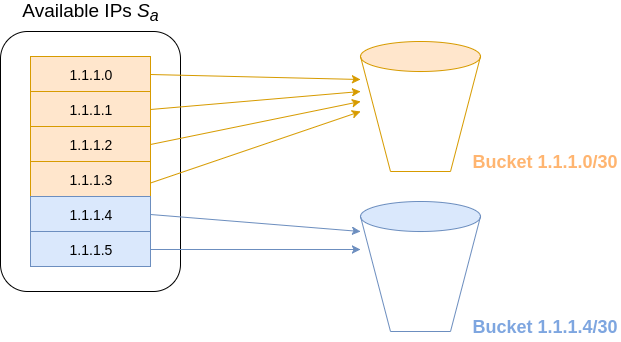
\includegraphics[width=0.8\textwidth]{renders/IpsByBucketSize4.png}
      \caption{Assigning IPs to Buckets with a Bucket Size of 4}
      \label{fig:exampleIpsByBucket4}
\end{figure}

As discussed, the bucket size will be an integral power of 2, but an important question is which integral power of 2. The algorithm starts by assigning the IPs to their buckets using a bucket size equal to the largest possible CIDR block that can be obtained for the given $t$, as discussed previously.

At this point, the algorithm begins to take shape. Consider the situation represented in \reffig{fig:exampleIpsByBucket4} along with a value of $t = 4$. The inital bucket size will be 4 and the presence of a filled bucket ($1.1.1.0/30$) indicates that a CIDR block of the bucket size can be created. Since the bucket size is equal to the desired number of IPs, the optimal choice is the $1.1.1.0/30$ block.

Next consider the situation represented in \reffig{fig:exampleIpsByBucket4} along with a value of $t = 6$. The initial bucket size will still be 4 (as this is the largest integral power of 2 smaller than $t$). Thus, the algorithm will again detect that the $1.1.1.0/30$ bucket is full and select this block of four IPs. However the algorithm must return a total of $t = 6$ IPs and therefore must select a further 2 IPs. The algorithm accomplishes this by making a recusrive call. By removing all of the (so far) selected IPs from the set of available IPs (forming the $S_a'$) and setting the new value of $t$ to be the remaning number of IPs required ($t'$), a recursive call will simply find the best set of IPs from what is left. This is shown in \reffig{fig:exampleIpsByBucket2} in which the recusrive call would return $1.1.1.4/31$ as this bucket is full. 

\begin{figure}[H]
      \centering
      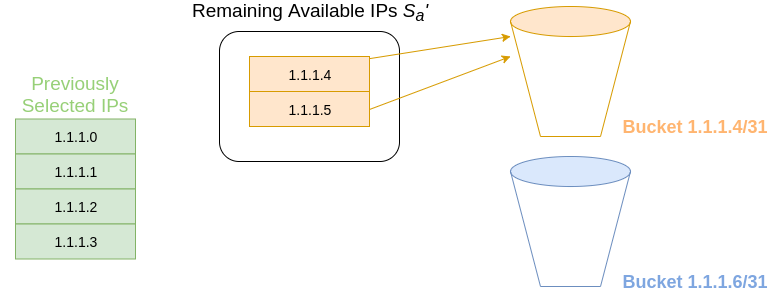
\includegraphics[width=0.8\textwidth]{renders/IpsByBucketSize2.png}
      \caption{Assigning Remaining IPs to Buckets with a Bucket Size of 2}
      \label{fig:exampleIpsByBucket2}
\end{figure}

In the case of $t = 7$, the algorithm would proceed as before, with one extra recusrive call with $t = 1$. Assuming there were sufficient IPs available (the number of IPs in the diagrams were limited for brevity), the algorithm would have selected the same 6 IPs as before and the final call would be the trivial case of $t = 1$ in which a random IP can be selected. At each stage, the set of IPs returned from the recusrive calls can then be unioned with the current call's chosen IPs, and the unioned set returned. 

The final possibility to consider is what should be done when no buckets are filled. In this case, the algorithm should not select any IPs at this bucket size. Instead, it should reduce the bucket size to the next highest integral of 2 and recurse, setting $t$ equal to this reduced bucket size. However, there is another important step, the need for which is best illustrated with an example. A diagram of this code path is shown in \reffig{fig:ipAlgTrickyCodePath}

If the initial value for $t$ is 6, the initial bucket size will be 4. If no buckets of size 4 are filled, the algorithm will then recurse. Let the total number of IPs requied that is used for this recusrive call be denoted as $t_1'$. Thus, for the recursive call, $t_1' = 2$ (the next largest integral power of 2 as discussed previously) and the set of available IPs is unchanged $S_{a_1} = S_a$. Let the set of chosen IPs returned from this first recursive call be denoted as $S_{c_1}$.

The initial call required 6 IPs to be returned, however this first recursive call will always return 2 IPs that should be used. Thus a second recursive call is required. Let the total number of IPs required that is used for this second recursive call be denoted as $t_2'$. $t_2'$ is calculated using the formula given in \refeq{eq:secondRecurseT2}. This is simply the remaining number of IPs that need to be chosen after the first recursive call. 

\begin{equation}\label{eq:secondRecurseT2}
t_2' = t - t_1'
\end{equation}

Finally, the set of available IPs that is used for the second recursive call ($S_{a_2}$) is given by \refeq{eq:availableIpsSecondRecurse}. This is the initial set of all available IPs, with the IPs chosen from the first recursive call ommited.

\begin{equation}\label{eq:availableIpsSecondRecurse}
S_{a_2} = S_a - S_{c_1}
\end{equation}

\begin{figure}[H]
      \centering
      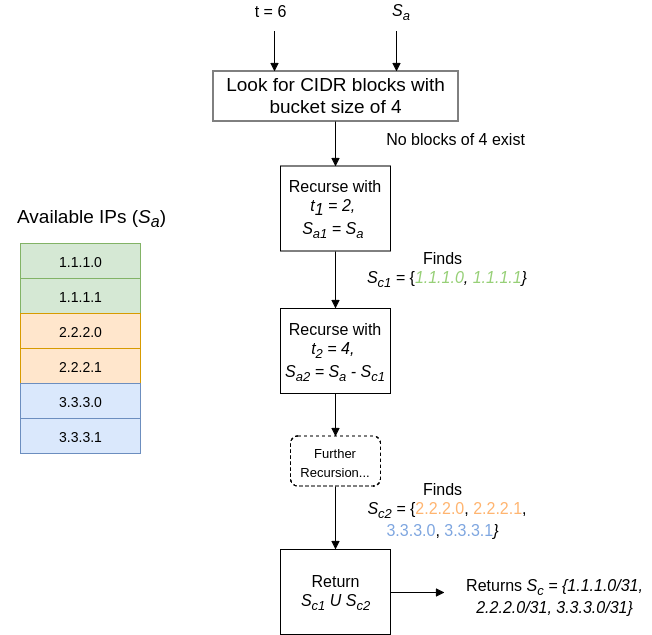
\includegraphics[width=0.8\textwidth]{renders/IpAlgTrickyCodePath.png}
      \caption{Code Path when Algorithm Does Not Find Full Bucket}
      \label{fig:ipAlgTrickyCodePath}
\end{figure}

The steps of the algorithm (for the simplified case of having no existing IPs) are shown in \ref{list:algSteps}:
\begin{itemize}\label{list:algSteps}
\item{Set bucket size to be largest integral power of 2 that is less than $t$}
\item{Assign all available IPs into buckets using the calculated bucket size}
\item{If a bucket is full}
  \begin{itemize}
  \item{Add all of the IPs in the bucket to the set of chosen IPs ($S_c$)}
  \item{Remove all of the IPs in the bucket from the set of available IPs (forms $S_a'$)}
  \item{Calculate $t'$ as $t - bucketSize$}
  \item{Recurse using $S_a'$ and $t'$ (if neccessary)}
  \end{itemize}
\item{Otherwise}
  \begin{itemize}
  \item{Recurse using next biggest integral power of 2 and the initial set of available IPs}
  \item{Recurse using the number of remaining IPs required and the set of available IPs, excluding those returned from the previous recursive call}
  \item{Return the union of the results of the two recursive calls.}
  \end{itemize}
\end{itemize}

\subsection{Implementing the Algorithm}
\subsection{Unit Testing the Algorithm}
%^ is pretty ropey, reread and make some adjustments before continuing with the alg

% CIDR notation works by specifying a bit mask that should be used for a logical $AND$ operation with the IP address. The bit masks are specified using the conventional slash notation. $/32$ implies that the bit mask contains 32 ones, $/31$ implies that the bit mask contains 31 ones and 1 zero (the zero being the least significant bit) and so on. 